%!TEX root = ../thesis.tex
%*******************************************************************************
%****************************** Seventh Chapter **********************************
%*******************************************************************************
\chapter{Reinforcement Learning in Electricity Markets}
\label{chapter:reinforcement}
% **************************** Define Graphics Path **************************
\ifpdf
    \graphicspath{{Chapter3/Figs/Raster/}{Chapter3/Figs/PDF/}{Chapter3/Figs/}}
\else
    \graphicspath{{Chapter3/Figs/Vector/}{Chapter3/Figs/}}
\fi


\section*{Prologue}

Test

\section{Introduction}

Test

\section{Literature review}

Test

\section{Carbon optimisation}

Test

\section{Conclusion}

Test








\begin{abstract}
	
	% Background
	
	Decentralized electricity markets are often dominated by a small subsection of generator companies, who control a majority of the capacity. In this paper, we explore the effect of the total controlled electricity capacity by any single or group of generator companies has on the average electricity price. To achieve this we use the deep deterministic policy gradient reinforcement learning algorithm to strategically bid in a uniform pricing electricity market. Where a uniform pricing market is one where all players are paid the highest accepted price. We utilize the agent-based model ElecSim, which is parameterized to the United Kingdom for the year 2018. 
	
	We find that capacity has an impact on average electricity price in a single year. If any one generator company, or a collaborating group of generator companies, control more than ${\sim}$11\% of generation capaicity, prices begin to increase by ${\sim}$25\%. The value of ${\sim}$25\% may vary between market structures and countries. Once the capacity controlled by a generator company is higher than ${\sim}$35\% of the total capacity, prices increase exponentially, leading to an almost tripling of average electricity price. The use of a market cap of approximately double the average market price has the effect of significantly decreasing this effect and maintaining a competitive market, irrespective of the capacity controlled by a single, or group of generator companies.
	
	% Methodology
	
	% Results
	
	
	
	
\end{abstract}


\section{Introduction}
\label{sec:introduction}

In this paper, we use a distributed monte-carlo simulation to model a decentralized electricity market. Decentralized electricity markets have a number of different market structures: day-ahead, balancing market and reserve markets. The day-ahead market settles payments for electricity for the following day. The balancing market is designed to regulate frequency of the market through matching supply and demand, whereas reserve markets provide capacity in case there are fluctuations in supply and demand, and electricity demand can't be matched with supply. Our model simulates a day-ahead market over a single year time period to explore the effects of market power on electricity prices.

Under perfectly competitive electricity markets, generator companies (GenCos) tend to bid their short-run marginal costs (SRMC) when bidding into the day-ahead electricity market. SRMC is the cost to produce a single MWh of electricity and excludes capital costs. However, electricity markets are often oligopolistic, where a small subset of GenCos provide the majority of the capacity to the market. Under these conditions, it is possible that the assumption that GenCos are price-takers does not hold. That is, large GenCos artificially increase the price of electricity to gain an increased profit using their market power. 

Reduced competition within electricity markets can lead to higher prices to the consumers, with no societal benefit. It is, therefore, within the interests of the consumer and that of government to maintain a competitive market. Low energy costs can enable innovation in other industries reliant on electricity, and in turn, make a more productive economy. Competition within electricity markets can be increased by only allowing single entities to have control over a small amount of electricity generation capacity.

In this paper, we explore the effect of total controlled capacity on electricity prices. Specifically, we allow different sizes of GenCos and groups of colluding GenCos, to bid strategically to maximize their profit using a reinforcement learning algorithm. This is in contrast to the strategy of bidding the SRMC of their respective power plants. For this, we use deep reinforcement learning (RL) to calculate a bidding strategy for GenCos in a day-ahead market. These GenCos are modelled as agents within the agent-based model, ElecSim \cite{Kell, Kell2020}. We use the UK electricity market instantiated on 2018 as a case study, similar to our work in \cite{Kell2019a}. That is, we model each GenCo with their respective power plants in the year 2018 to 2019. In total, we model 60 GenCos with 1085 power plants.

We use the deep deterministic policy gradient (DDPG) deep RL algorithm, which allows for a continuous action space \cite{Hunt2016}. Conventional RL methods require discretization of state or action spaces and therefore suffer from the curse of dimensionality \cite{Ye2020a}. As the number of discrete states and actions increases, the computational cost grows exponentially. However, too small a number of discrete states and actions will reduce the information available to the GenCos, leading to sub-optimal bidding strategies. Additionally, by using a continuous approach, we allow for GenCos to consider increasingly complex bidding strategies. 

Other works have considered a simplified model of an electricity market by modelling a small number of GenCos or plants \cite{EsmaeiliAliabadi2017,Tellidou2007}. We, however, model each GenCo as per the UK electricity market with their respective power plants in a day-ahead market. In addition, further work focuses on a bidding strategy to maximize profit for a GenCo. However, in our work, we focus on the impact that large GenCos, or colluding groups of GenCos, can have on the overall electricity price.


Our approach does not require GenCos to formulate any knowledge of the data which informs the market clearing algorithm or rival GenCo bidding strategies, unlike in game-theoretic approaches \cite{Wang2011}. This enables a more realistic simulation where the strategy of rival GenCos are unknown.

In Section \ref{sec:lit-review} we review the literature, and explore other approaches of RL in electricity markets. In Section \ref{sec:material} we introduce the agent-based model used and the DDPG algorithm. Section \ref{sec:methodology} explores the methodology taken for our case study. We discuss and conclude our work in Sections \ref{sec:discussion} and \ref{sec:conclusion} respectively. 




%- Why the current approaches / systems don't solve the problem

%- What is the innovation in this work

%- A short description of the solution

%- What are the key take-home messages

% Contributions of this work

%- Look at market power of individual or groups of agents

%- Outline of the rest of the work




\section{Literature Review}
\label{sec:lit-review}

Intelligent bidding strategies for day-ahead electricity markets can be divided into two broad categories: game-theoretic models and simulation. Agent based models (ABMs) allow for the simulation of heterogenous irrational actors with imperfect information. Additionally, ABMs allow for the modelling of the learning and adaption within a dynamic environment \cite{EsmaeiliAliabadi2017}. Game-theoretic approaches may struggle in complex electricity markets where Nash equilibriums do not exist \cite{Wang2011}.

Here, we explore game-theoretic approaches. Kumar \textit{et al.} propose a Shuffled Frog Leaping Algorithm (SFLA) \cite{VijayaKumar2014} to find bidding strategies for GenCos in electricity markets. SFLA is a meta-heuristic that is based on the evolution of memes carried by active individuals, as well as a global exchange of information among the frog population. They test the effectiveness of the SFLA algorithm on an IEEE 30-bus system and a practical 75-bus Indian system. A bus in a power system is a vertical line which several components are connected in a power system. For example generators, loads, and feeders can all be connected to a bus. They find superior results when compared to particle swarm optimization and the genetic algorithm with respect to total profit and convergence with CPU time. They assume that each GenCo bids a linear supply function, and they model the expectation of bids from rivals as a joint normal distribution. In contrast to their work, we do not require an estimation of the rivals bids.

Wang \textit{et al.} propose an evolutionary imperfect information game approach to analyzing bidding strategies with price-elastic demand \cite{Wang2011}. Their evolutionary approach allows for GenCos to adapt and update their beliefs about an opponents' bidding strategy during the simulation. They model a 2-bus system with three GenCos. Our work, however, models a simulation with 60 GenCos across the entire UK, which would require a 28-bus system model \cite{Bell2010}. 

Next, we explore reinforcement learning approaches used to make intelligent bidding decisions in electricity markets. RL is a suitable method for analyzing the dynamic behaviour of complex systems with uncertainties. RL can therefore be used to identify optimal bidding strategies in energy markets \cite{Yang2020}. Simulations are often used to provide an environment for the reinforcement learning algorithm. In the following papers discussed, simulations are used as the environment.


Aliabadi \textit{et al.} utilize an ABM and the Q-learning algorithm to study the impact of learning and risk aversion on GenCos in an oligopolistic electricity market with five GenCos \cite{EsmaeiliAliabadi2017}. They find that some level of risk aversion is beneficial, however excessive risk degrades profits by causing an intense price competition. Our paper focuses on the impact of the interaction of many GenCos within the UK electricity market. In addition, we extend the Q-learning algorithm to use the DDPG algorithm, which uses a continuous action space.

Bertrand \textit{et al.} use RL in a continuous intraday market. Specifically, they use the REINFORCE algorithm to optimize the choice of price thresholds. They demonstrate an ability to outperform the traditionally used method, the rolling intrinsic method, by increasing profit per day by 4.2\%. The rolling intrinsic method accepts any trade, which gives a positive profit if the contracted quantity remains in the bounds of capacity. In our paper, we model a day-ahead market and use a continuous action for price bids, as opposed to a discrete threshold.

Ye \textit{et al.} propose a novel deep RL based methodology which combines the DDPG algorithm with a prioritized experience replay (PER) strategy. The PER samples from previous experience, but samples from the ``important'' ones more often \cite{Schaul2016}. They use a day-ahead market as a case study with hourly resolution and show that they are able to achieve approximately 41\%, 20\% and 11\% higher profit for the GenCo than the MPEC, Q-learning and DQN methods, respectively. In our paper, we instead look at how to prevent GenCos (or sets of colluding GenCos) from forcing higher prices above market rates.



Zhao \textit{et al.} propose a modified RL method, known as the gradient descent continuous Actor-Critic (GDCAC) algorithm \cite{Zhao2016}. This algorithm is used in a double-side day-ahead electricity market simulation. Where in this case, a double-side day-ahead market refers to GenCos selling their supply to distribution companies, retailers or large consumers. Their approach performs better in terms of participant's profit or social welfare compared with traditional table-based RL methods, such as Q-Learning. Our work also looks at improving on table-based methods by using function approximators.





\section{Methodology}
\label{sec:material}

In this section we describe the RL methodology used for the intelligent bidding process as well as the simulation model used as the environment.

\subsection{Reinforcement Learning background}

%\subsubsection{RL Background}

In RL an agent interacts with an environment to maximize its cumulative reward. RL can be described as a Markov Decision Process (MDP). An MDP includes a state space $\mathcal{S}$, action space $\mathcal{A}$, a transition dynamics distribution $p(s_{t+1}|s_t,a_t)$ and a reward function, where $r:S\times \mathcal{A} \rightarrow \mathbb{R}$. At each time step an agent receives an observation which is used to modify the agent's behaviour.

An agent's behaviour is defined by a policy, $\pi$. $\pi$ maps states to a probability distribution over the actions $\pi:\mathcal{S}\rightarrow \mathcal{P}(\mathcal{A})$. The return from a state is defined as the sum of discounted future reward $R_t=\sum_{i=t}^T\gamma^{(i-t)}r(s_i,a_i)$. Where $\gamma$ is a discounting factor $\gamma \in [0,1]$. The return is dependent on the action chosen, which is dependent on the policy $\pi$. The goal in reinforcement learning is to learn a policy that maximizes the expected return from the start distribution $J=\mathbb{E}_{r_i,s_i \sim E,a_i \sim \pi}[R_1]$. 

The expected return after taking an action $a_t$ in state $s_t$ after following policy $\pi$ can be found by the action-value function. The action-value function is used in many reinforcement learning algorithms and is defined in Equation \ref{eq:action-value}.

\begin{equation}
\label{eq:action-value}
Q^{\pi}(s_t,a_t)=\mathbb{E}_{r_{i\geq t},s_{i>t}\sim \mathcal{E},a_{i>t}\sim\pi}[R_t|s_t,a_t]
\end{equation}

The action-value function defines the expected expected reward at time $t$, given a state $s_t$ and action $a_t$ when following the policy $\pi$.

\subsection{Q-Learning}

An optimal policy can be derived from the optimal $Q$-values $Q_*(s_t,a_t)=\max_\pi Q_\pi(s_t,a_t)$ by selecting the action corresponding to the highest Q-value in each state.

Many approaches in reinforcement learning use the recursive relationship known as the Bellman equation, as defined in Equation \ref{eq:bellman}:

\begin{dmath}
	\label{eq:bellman}
	Q^\pi(s_t,a_t)=\mathbb{E}_{{r_t},s_{t+1}\sim E} [r(s_t,a_t)+
	\gamma\mathbb{E}_{a_{t+1}\sim \pi}[Q_\pi(s_{t+1},\pi(s_{t+1}))]].
\end{dmath}

\noindent The Bellman equation is equal to the action which maximises the reward plus the discount factor multiplied by the next state's value, by taking action the action after following the policy in state $s_{t+1}$ or $\pi(s_{t+1})$.

The Q-value can therefore be improved by bootstrapping. This is where the current value of the estimate of $Q_\pi$ is used to improve its future estimate, using the known $r(s_t,a_t)$ value. This is the foundation of Q-learning \cite{Gay2007}, a form of \textit{temporal difference} (TD) learning \cite{Sutton2015}, where the update of the Q-value after taking action $a_t$ in state $s_t$ and observing reward $r_t$, which results in state $s_{t+1}$ is:
\begin{equation}
Q(s_t,a_t)\leftarrow Q(s_t,a_t)+\alpha\delta_t
\end{equation}

\noindent where,

\begin{equation}
\delta_t=r_t+\gamma\max_{a_{t+1}}Q(s_{t+1},a_{t+1})-Q(s_{t},a_t)
\end{equation}

\noindent $\alpha\in [0,1]$ is the step size, $\delta_t$ represents the correction for the estimation of the Q-value function and $r_t+\gamma\max_{a_{t+1}}Q(s_{t+1},a_{t+1})$ represents the target Q-value at time step $t$.	


It has be proven that if the Q-value for each state action pair is visited infinitely often, the learning rate $\alpha$ decreases over time step $t$, then as $t\rightarrow \infty$, $Q(s,a)$ converges to the optimal $Q_*(s,a)$ for every state-action pair \cite{Gay2007}.

However, it is often the case that Q-learning suffers from the curse of dimensionality. This is because Q-learning stores the Q-value function in a look-up table. This therefore requires the action and state spaces to be discretized. As the number of discretized states and actions increases, the computational cost increases exponentially, making the problem intractable. 

\subsection{Deep Deterministic Gradient Policy}


It is not straightforward to apply Q-learning to continuous action spaces. This is because in continuous spaces, finding the greedy policy requires an optimization of $a_t$ at every time step. Optimizing for $a_t$ at every time step would be too slow to be practical with large, unconstrained function approximators and nontrivial action spaces \cite{Hunt2016}. To solve this, an actor-critic approach based on the deterministic policy gradient (DPG) algorithm is used \cite{Silver2014}.


The DPG algorithm maintains a parameterized actor function $\mu(s|\theta^\mu)$ which specifies the current policy by deterministically mapping states to a specific action. The critic $Q(s,a)$ is learned using the Bellman equation as in Q-learning. The actor is updated by applying the chain rule to the expected return from the start distribution $J$ with respect to the actor parameters:

\begin{align}
\begin{split}
\triangledown_{\theta^\mu}J\approx\mathbb{E}_{s_t\sim\rho^\beta}[\triangledown_{\theta^\mu}Q(s,a|\theta^Q)|_{s=s_t,a=\mu(s_t|\theta^\mu)}] \\
= \mathbb{E}_{s_t\sim\rho^\beta}[\triangledown_aQ(s,a|\theta^Q)|_{s=s_t,a=\mu(s_t)}\triangledown_{\theta_\mu}\mu(s|\theta^\mu)|_{s=s_t}]
\end{split}
\end{align}

This is the policy gradient. The policy gradient is the gradient of the policy's performance. The policy gradient method optimizes the policy directly by updating the weights, $\theta$, in such a way that an optimal policy is eventually found. This is achieved by performing gradient ascent on the policy and its parameters $\pi^\theta$.

Introducing non-linear function approximators, however, means that convergence is no longer guaranteed. Although, these function approximators are required in order to learn and generalize on large state spaces. The Deep Deterministic Gradient Policy (DDPG) modifies the DPG algorithm by using neural network function approximators to learn large state and action spaces online.

A replay buffer is utilized in the DDPG algorithm to address the issue of ensuring that samples are independently and identically distributed. The replay buffer is a finite sized cache, $\mathcal{R}$. This is where transitions are samples from the environment through the use of the exploration policy, and the tuple $(s_t,a_t,r_t,s_{t+1})$ is stored in the replay buffer. Old samples are discarded as the replay buffer becomes full. The actor and critic are trained by sampling from the replay buffer uniformly. 

A copy is made of the actor and critic networks, $Q'(s,a|\theta^{Q'})$ and $\mu'(s|\theta^{\mu'})$ respectively. These are used for calculating the target values. To ensure stability, the weights of these target networks are updated by slowly tracking the learned networks.

\begin{algorithm}
	\caption{DDPG Algorithm \cite{Hunt2016}}
	\begin{algorithmic}[1]
		\footnotesize
		\State Initialize critic network $Q(s,a|\theta^Q)$ and actor $\mu(s|\theta^\mu)$ with random weights $\theta^Q$ and $\theta^\mu$
		\State Initialize target network $Q'$ and $\mu'$ with weights $\theta^{Q'}\leftarrow\theta^Q,\theta^{\mu'}\leftarrow \theta^{\mu}$
		\State Initialize replay buffer $R$
		\For{\texttt{episode=1,M}}
		\State Initialize a random process $\mathcal{N}$ for action exploration
		\State Receive initial observation state $s_1$
		\For{\texttt{t=1,T}}
		\State Select action $a_t=\mu(s_t|\theta^{\mu})+\mathcal{N}_t$ according to the policy and exploration noise, $\mathcal{N}_t$
		\State Execute action $a_t$ and observe reward $r_t$ and new state $s_{t+1}$
		\State Store transition $(s_t, a_t, r_t, s_{t+1})$ in $R$
		\State Sample a random minibatch of $N$ transitions $(s_i, a_i, r_i, s_{i+1})$ from $R$
		\State Set $y_i=r_i+\gamma Q'(s_{i+1},\mu'(s_{i+1},\mu'(s_{i+1}|\theta^{\mu'})|\theta^{Q'})$
		\State Update critic by minimizing the loss: $$L=\frac{1}{N}\sum_i(y_i-Q(s_i,a_i|\theta^Q))^2$$
		\State Update the actor policy using the sampled policy gradient: $$\triangledown_{\theta^\mu}J\approx \frac{1}{N}\sum_i\triangledown_a Q(s,a|\theta^Q)|_{s=s_i,a=\mu(s_i)}\triangledown_{\theta^\mu}\mu(s|\theta^\mu)|_{s_i}$$
		\State Update the target networks:
		$$\theta^{Q'}\leftarrow\tau\theta^Q+(1-\tau)\theta^{Q'}$$
		$$\theta^{\mu'}\leftarrow\tau\theta^\mu+(1-\tau)\theta^{\mu'}$$
		\EndFor
		\EndFor
	\end{algorithmic}
\end{algorithm}

\subsection{Simulation}

For this work, we utilized the long-term electricity market agent-based model, ElecSim \cite{Kell,Kell2020b}. The model was run using a short term approach by only iterating through a single year (2018), composed of eight representative days, each of 24 time steps.

ElecSim is made up of six fundamental components: 1) power plant data; 2) scenario data; 3) the time steps of the algorithm; 4) the power exchange; 5) the investment algorithm and 6) the generation companies (GenCos) as agents. For this paper we ignore the investment algorithm, due to investments happening only once a year, and not in the first year of operation. 

ElecSim uses a subset of representative days of electricity demand, solar irradiance and wind speed to approximate a full year. Representative days, in this context, are a subset of days which can closely approximate an entire year's electricity demand and weather patterns. By using a subset, we are able to reduce the computational time to run, whilst maintaining accuracy of modelling the real electricity market \cite{Kell2020}.

Figure \ref{fig:model_details} shows how the six fundamental components interact. The electricity demand is matched with the supply of the power plants, owned by the generator companies (GenCos). We have configured ElecSim to model the UK electricity market, using the configuration file. Specifically, we model the actual GenCos with their respective power plants that were in operation in 2018.



\begin{figure}
	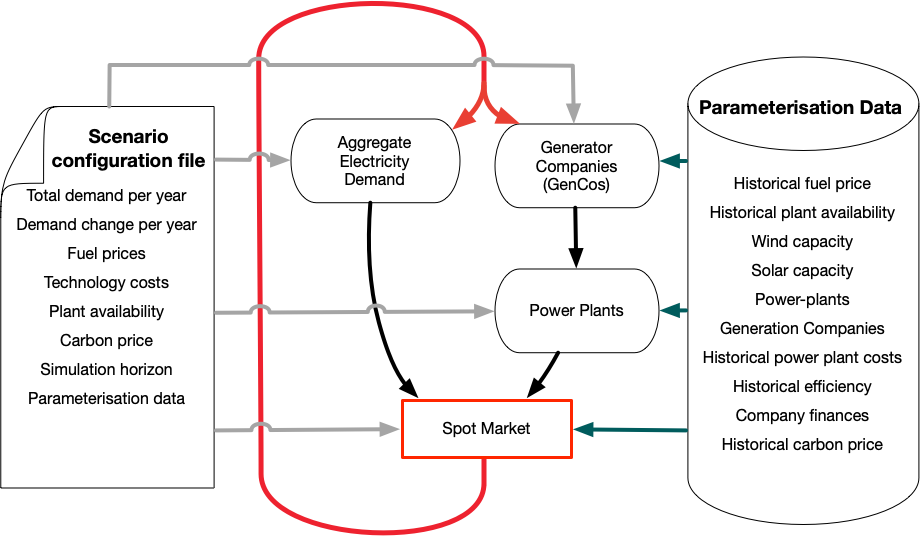
\includegraphics[width=0.44\textwidth]{figures/methedology/system-overview-v2}
	\caption{System overview of ElecSim \cite{Kell}.}
	\label{fig:model_details}
\end{figure}

The market has a uniform pricing bidding mechanism. A uniform pricing mechanism is one where a single price is paid for all electrical capacity, irrespective of the bid. The bid that is paid is that of the highest accepted price. This incentivises GenCos to bid their SRMC. SRMC is the price that it takes to generate a single MWh of electricity, excluding capital costs. 

In this work we modify the bidding strategy of a subset of the GenCos. They bid based upon the policy of the DDPG RL algorithm, as opposed to their SRMC. This is to explore whether large GenCos, or a group of GenCos can manipulate the price of the electricity market through market power. The remaining GenCos, which fall outside of this group, maintain a bidding strategy based upon their SRMC.

For the purpose of this work we do not consider flow constraints within the electricity mix. This is because we model the entire UK with 1000+ generators, and many nodes and buses. This would make the optimization problem intractable for the purpose of our simulation, especially when considering the many episodes required for training. It takes ${\sim}125$ seconds to run a single year in the simulation, or episode with our current setup. By increasing the simulation time further, we would make the compute time intractable due to the many episodes required for reinforcement learning to learn an effective policy.




%- Market Structure of ElecSim (yearly outlook) \\
%- Real life structure of the UK\\

%- We change the price of the bid (from SRMC to Bid cap in the market)\\

%- Do not consider flow constraints due to the large nature of the simulation\\
%- Amount of time taken to run 1 episode is...\\ 




\section{Experiment Setup}
\label{sec:methodology}


To parameterize the simulation we use data from the United Kingdom in 2018. This included 1085 electricity generators and power plants with their respective GenCos. The data for this was taken from the BEIS DUKES dataset \cite{dukes_511}. The electricity load data was modelled using data from \cite{gridwatch}, offshore, and onshore wind and solar irradiance data was taken from \cite{Pfenninger2016}.

We changed the bidding strategy of the selected GenCos, as well as groups of GenCos, from a bid based upon the SRMC to a policy defined by the DDPG RL algorithm. Through this we hoped to observe the ability for RL to find the point at which market power  artificially inflates electricity prices. To achieve this, we chose the six largest GenCos in the UK, as well as a smaller GenCo as a control. Table \ref{table:genco_table} displays the groups of GenCos, as well as individual GenCos, with their respective capacity and number of plants.





\begin{table}
	\renewcommand{\arraystretch}{1.5}
	\centering
	\begin{tabular}{p{5cm}lllp{1.5cm}}
		\toprule
		GenCo Groups                                                                                                                  & Capacity & Num. of Plants \\ \midrule
		Orsted                                                                                                                       & 2738.7   & 11               \\
		Drax Power Ltd                                                                                                               & 4035.0   & 3                \\
		Scottish power                                                                                                               & 4471.5   & 49               \\
		Uniper UK Limited                                                                                                            & 6605.0   & 9                \\
		SSE                                                                                                                          & 8390.7   & 130              \\
		RWE Generation SE                                                                                                            & 8664.0   & 11               \\
		EDF Energy                                                                                                                   & 14763.0  & 14               \\
		\{EDF Energy, RWE Generation SE\}                                                                                              & 23427.0  & 25               \\
		\{EDF Energy, \\ RWE Generation SE, SSE\}                                          & 31817.7  & 155              \\
		\{EDF Energy, \\ RWE Generation SE, SSE, Uniper UK Ltd\}                              & 38422.7  & 164              \\
		\{EDF Energy, \\ RWE Generation SE, SSE, Uniper UK Ltd, Scottish Power\}              & 42894.2  & 213              \\
		\{EDF Energy, \\ RWE Generation SE, SSE, Uniper UK Ltd, Scottish Power, Drax Power Ltd\} & 46929.2  & 216              \\ 
		\bottomrule
	\end{tabular}
	\bigskip
	\caption{Groups of GenCos that used bidding strategies, number of plants and total electricity generting capacity owned.}
	\label{table:genco_table}
\end{table}


For the reinforcement learning problem we have the following tuple: $(s_t,a_t,r_t,s_{t+1})$, where $(s_t, s_{t+1})$ is the state at time $t$ and $t+1$ respectively, $a_t$ is the action at time $t$ and $r_t$ is the reward at time $t$. For our problem the state space is given by the tuple shown in Equation \ref{eq:observation_tuple}:

\begin{equation}
\label{eq:observation_tuple}
s_t=(H_i,D_i,p_{C02},p_{gas},p_{coal},p_{c})
\end{equation}

\noindent where $H_i$ is the segment hour to bid into at timestep $i$, $D_t$ is the demand of the segment hour at timestep $t$, $p_{gas}$ is the price of gas, $p_{C02}$ is the carbon tax price, and $p_{c}$ is the clearing price. We set the reward, $r_t$ to be the average electricity price of that time step, $p_{avg}$.

For the action space, $a_t$, we modelled two scenarios. Where there was a price cap of \textsterling$150$/MWh and \textsterling$600$/MWh. Only these two values were chosen to reduce computational load. We chose \textsterling$150$/MWh as a reasonable price cap that may be introduced by a Government, which allowed for variations in demand within different demand segments. The $\textsterling 600$/MWh was chosen to simulate an unbounded price cap. This enabled us to see the price that an equilibrium is reached within a market with agents with market power. 

For this work, we assume that the action space $a_t$ only bids price, and not how much capacity to bid on the market. We assume this to reduce the dimensionality of $a_t$, and simplify the training process.

In this work, we assume that the GenCo Groups have no information about the generation capacity, marginal cost, bid prices or profits of other GenCos \cite{EsmaeiliAliabadi2017}. They learn the maximum profit that can be made through experience within a particular market.

%- Grouping agents based upon size and seeing results\\
%- Observation and action space \\
%- Allowing them to bid maximum of \textsterling600 and a market cap of \textsterling150
%- Assumed that all capacity is bid\\
%- Explore our parameters of DDPG

%- The GenCo has no information about the generation capacity, marginal cost, bid prices or profits of other GenCos, or the total number of GenCos in the system. \cite{EsmaeiliAliabadi2017}\\



%-Note that in the model, the GenCo does not take any strategic action, that is, the GenCo does not consider the actions of other GenCos explicitly in its decision process. In fact, it does not have information on other GenCos. The GenCo is modeled as a simple agent that learns only from its own experi- ence. GenCos’ collective behavior, however, may lead to strategic outcomes.\cite{EsmaeiliAliabadi2017}\\




\section{Results}
\label{sec:results}

In this section we detail the results of the RL algorithm, and the effect that capacity has on average electricity price within the UK.

Figures \ref{fig:unbounded_timesteps} and \ref{fig:bounded_timesteps} show the rewards over number of time steps for the unbounded and bounded cases respectively. Figure \ref{fig:unbounded_timesteps} shows a clear difference between agents which use the DDPG RL strategy and have a large capacity (green and yellow) compared to those which have a smaller capacity (dark purple). The axis in Figure \ref{fig:unbounded_timesteps} are much larger than those of \ref{fig:bounded_timesteps}, highlighting the effect of market power on an unbounded market.

The average electricity price for a capacity below 30,000MW, or ${\sim35\%}$ of total capacity, remains stable between \textsterling70/MWh and \textsterling100/MWh. This range may be due to the stochasticity in calculating the weights for the DDPG algorithm. The average electricity price does not change over the time steps or training. We therefore hypothesize that there is no market power as long as an individual GenCo owns below ${\sim35\%}$ of total electrical capacity. 

On the other hand, once the capacity of a GenCo or groups of GenCos is above 30,000MW, there is a significant increase in the average electricity price for capacity. The average electricity price for capacity falls between the range of  \textsterling$170$/MWh and \textsterling$220$/MWh. The electricity price is low at the start of training, and ends high, which suggests that the RL strategy has learnt a method of gaining a higher reward.




\begin{figure}
	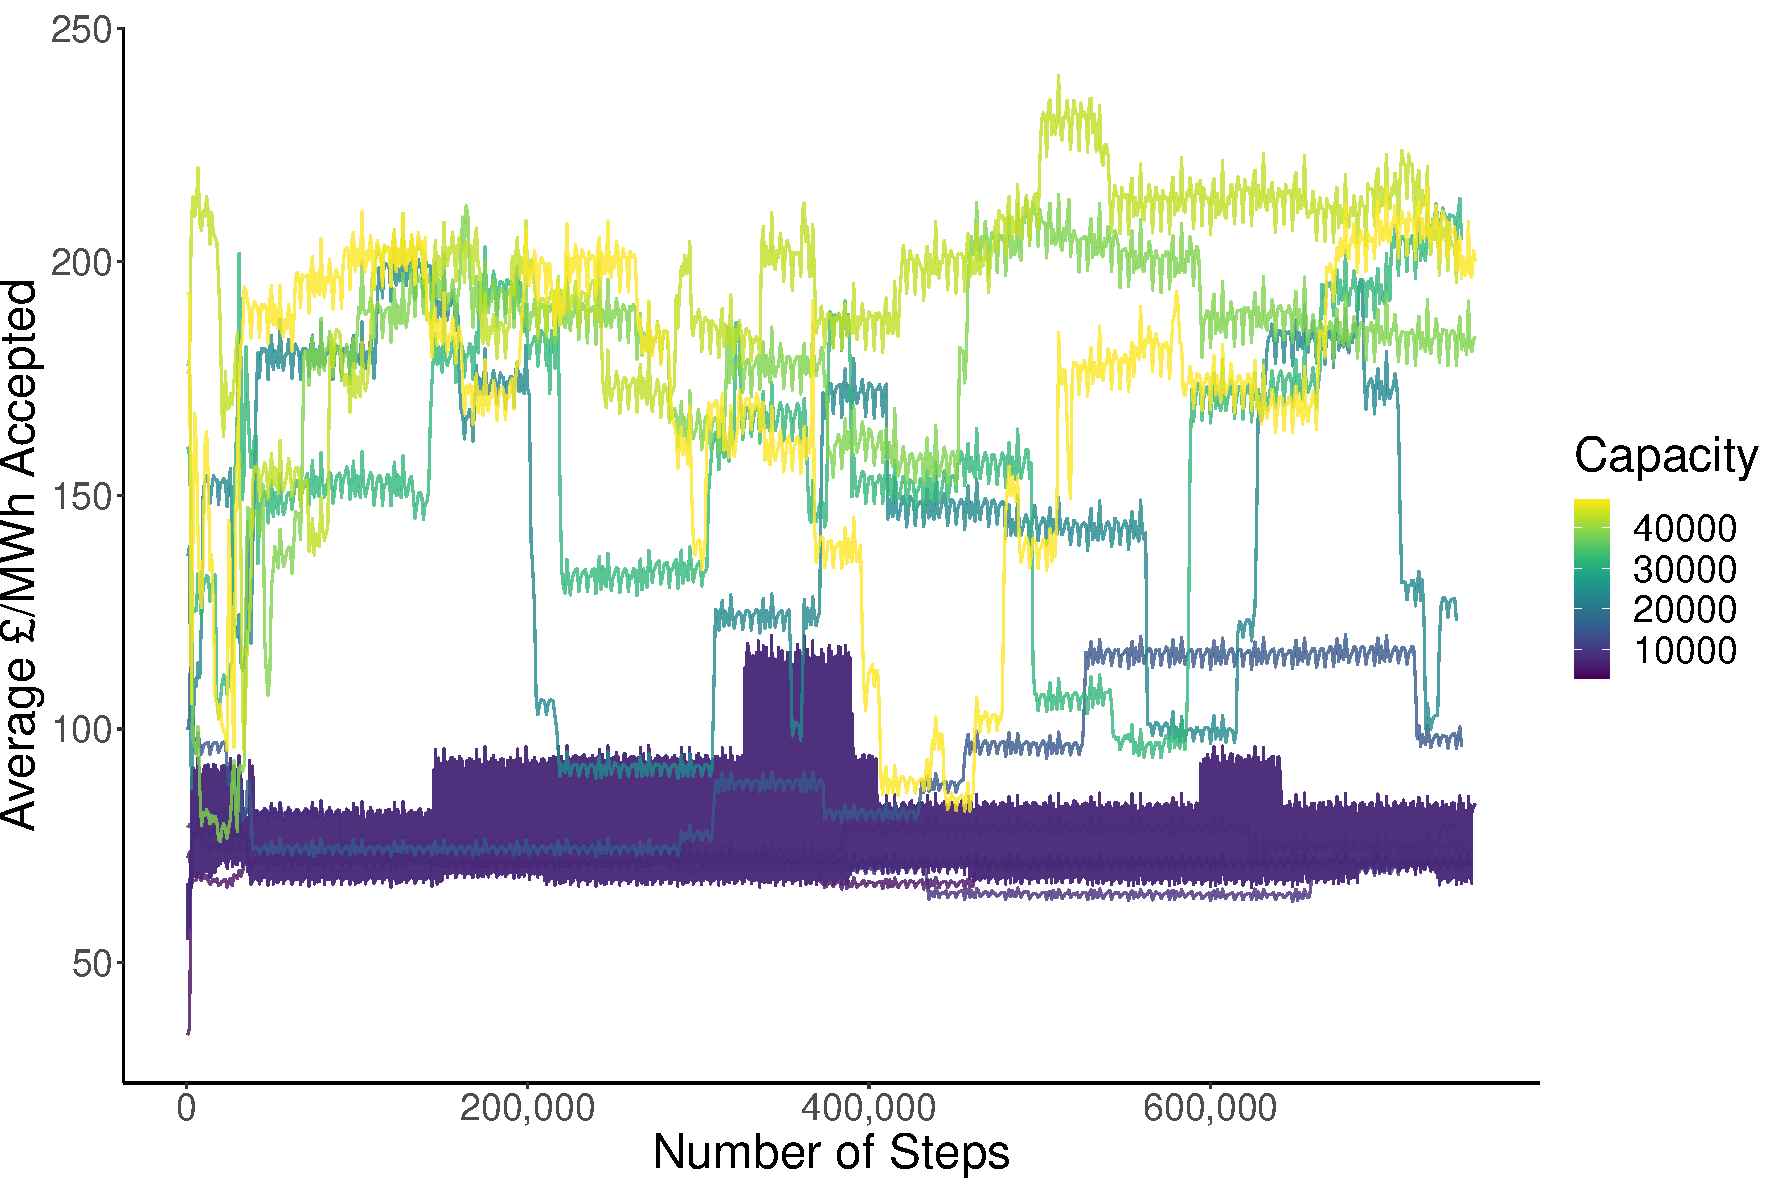
\includegraphics[width=0.48\textwidth]{figures/results/unbounded_results.pdf}
	\caption{Reward over time for different groups of GenCos, max bid = \textsterling $600$/MWh.}
	\label{fig:unbounded_timesteps}
\end{figure}


Figure \ref{fig:unbounded_results_scatter} displays the capacity of agents that use the RL strategy versus average electricity price for the unbounded case. The color displays the number of steps. The step-change as shown in Figure \ref{fig:unbounded_timesteps} can be seen clearly here, with agents with a capacity larger than ${\sim}$25,000MW causing a step change in electricity price. Electricity prices seems to cluster below ${\sim}$10,000MW. However, after this point the average electricity price begins to increase.



\begin{figure}
	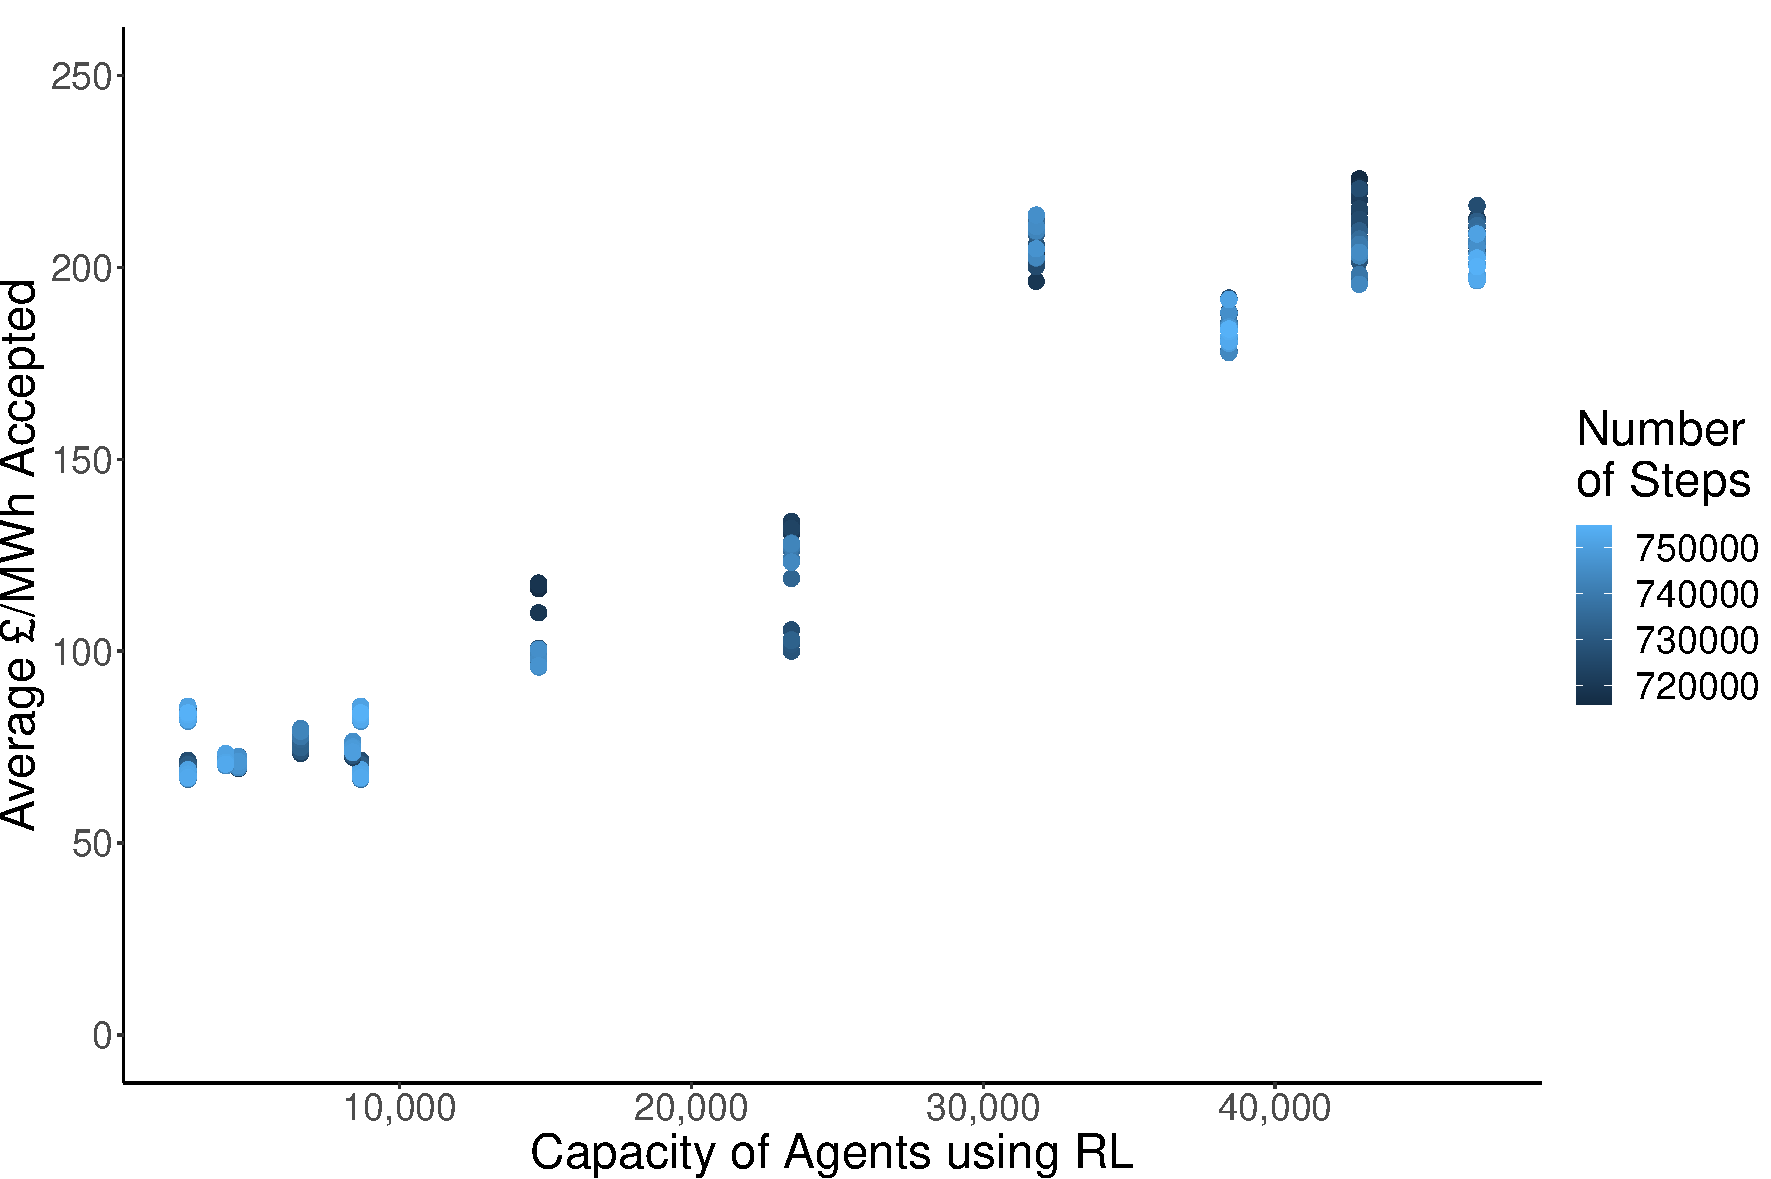
\includegraphics[width=0.48\textwidth]{figures/results/unbounded_results_scatter.pdf}
	\caption{Capacity of agents using RL vs. average electricity price accepted, for unbounded agents.}
	\label{fig:unbounded_results_scatter}
\end{figure}



Figure \ref{fig:bounded_timesteps} shows a cluster between ${\sim}$\textsterling$60$/MWh and ${\sim}$\textsterling$80$/MWh irrespective of the capacity of the agents. This is verified by Figure \ref{fig:bounded_results_scatter}. This seems to suggest that setting a lower market cap reduces the ability for even large generators from influencing the electricity price.


\begin{figure}
	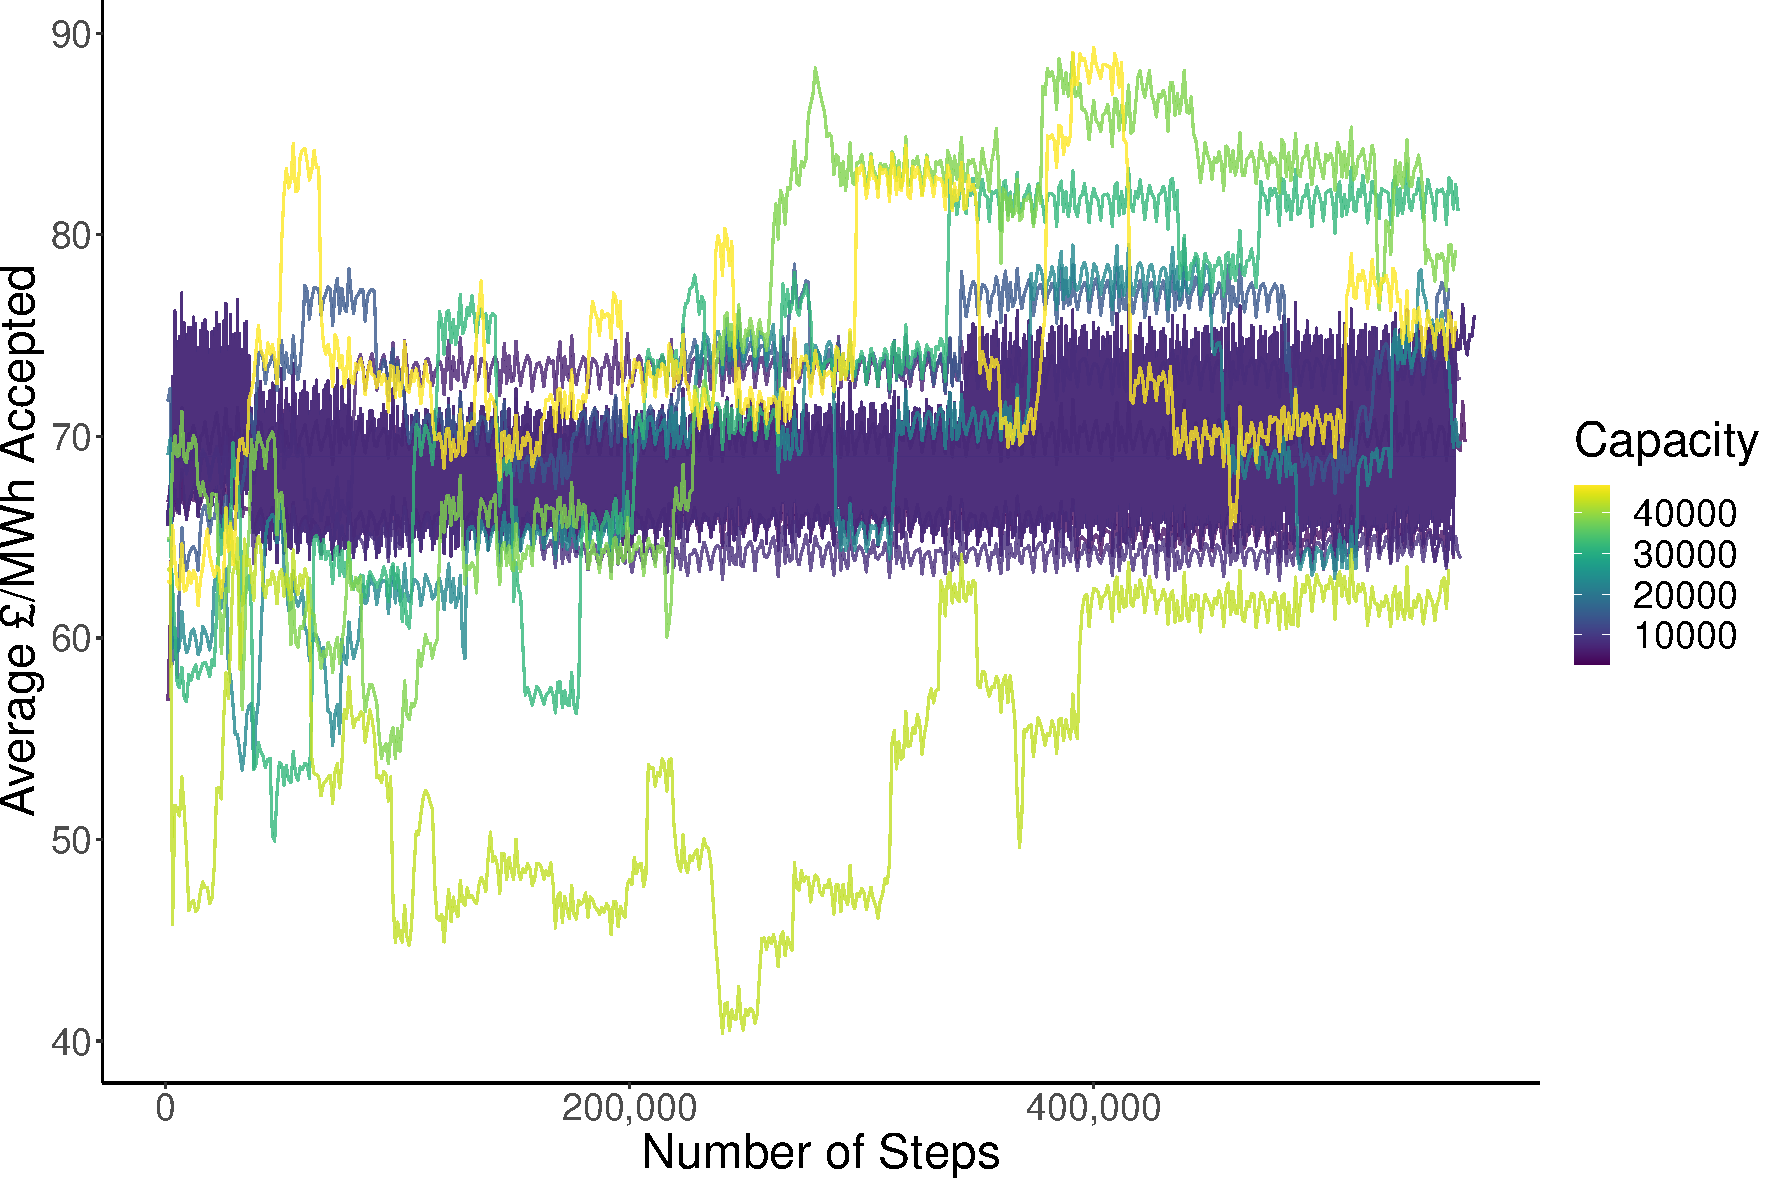
\includegraphics[width=0.48\textwidth]{figures/results/bounded_results.pdf}
	\caption{Reward over time for different groups of GenCos, max bid = \textsterling $150$/MWh.}
	\label{fig:bounded_timesteps}
\end{figure}




\begin{figure}
	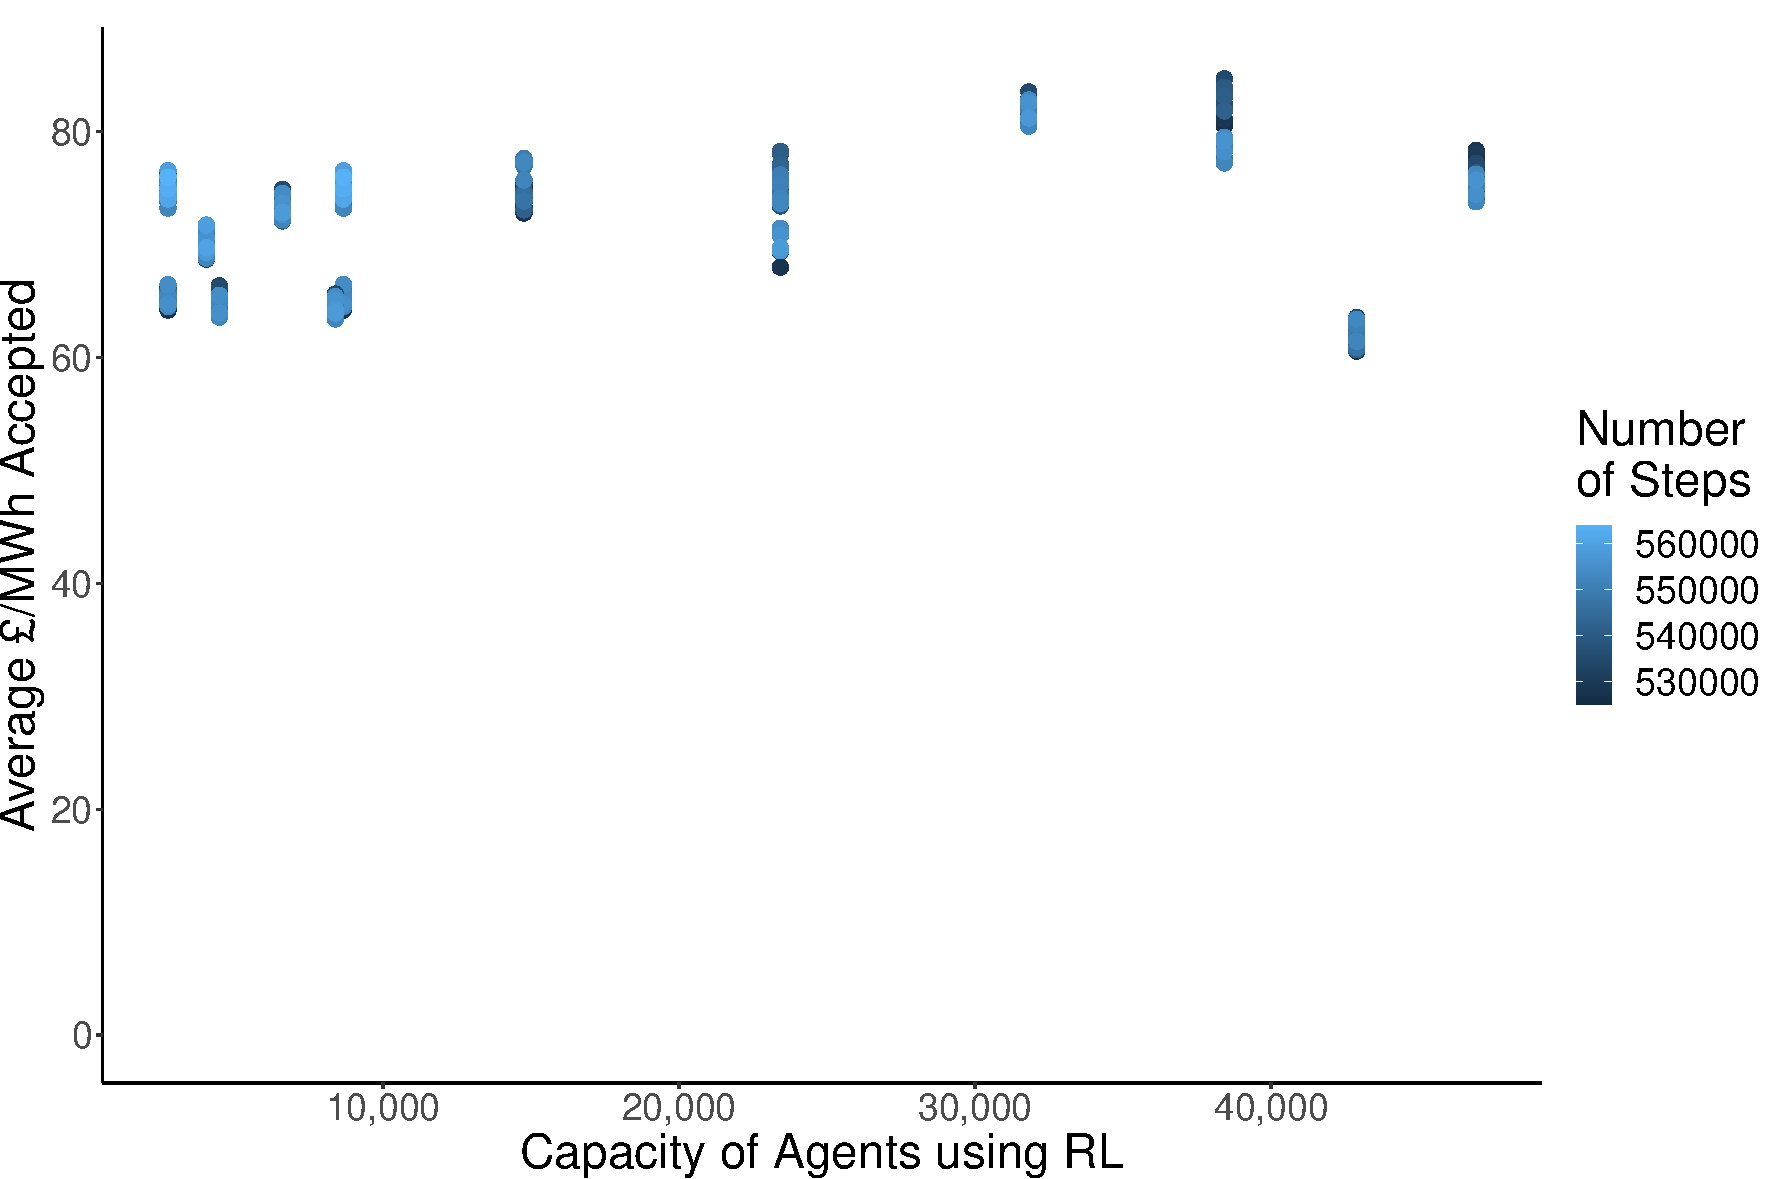
\includegraphics[width=0.48\textwidth]{figures/results/bounded_results_scatter.pdf}
	\caption{Capacity of agents using RL vs. average electricity price accepted, for bounded agents.}
	\label{fig:bounded_results_scatter}
\end{figure}





%- Show time steps vs. reward for both scenarios \\
%- Show the step change in reward after a certain amount of controlled capacity

\section{Discussion}
\label{sec:discussion}

Our results demonstrate the ability for GenCos to artificially increase the electricity price through market power in an uncapped market. Our results have shown that in an uncapped market, any one agent or groups of agents who make bids using the same strategy and information, should have less than ${\sim}$10,000MW. This defines the optimal capacity by any one GenCo to have a fair level of competition. After this, the electricity price begins to rise with the same outcome and welfare.

However, if there is an electricity market with a few large or colluding players, it is possible to remove their advantage through the introduction of a price cap. Our results show no significant difference in price at any levels of capacity if a market cap of \textsterling$150$ is introduced.

This information and approach can help to inform governmental policy to ensure fair competition within electricity markets. It is hypothesised that the findings in this paper are generalizable to other decentralized electricity markets in other geographies due to their similar market structures. Whilst the figures presented here may not be the same, we hypothesise that the region of interest will be similar.


%- Make suggestions based upon optimal level of competition \\
%- Importance of understanding market power and having a regulator otherwise prices can significantly increase

\section{Conclusion}
\label{sec:conclusion}

In this work we used the deep deterministic policy gradient (DDPG) reinforcement learning method to make strategic bids within an electricity market. We utilized the agent-based model ElecSim to model the UK electricity market. We utilized the DDPG algorithm only for a certain subset of agents, from small individual generation companies (GenCos) to large groups of GenCos. 

This enabled us to explore ability for GenCos with a large capacity to artificially increase the price of electricity market within the UK if they are in control of a sufficiently large electricity generation capacity. Our results show that the optimum level of control of any one GenCo or groups of GenCo is below ${\sim}10,000$MW or ${\sim}$11\% of the total capacity. Above this, prices begin to increase with no real additional benefit to the consumer. After ${\sim}$25,000MW the prices begin to increase substantially, to ${\sim}$\textsterling200, over triple the original cost without this market power. The introduction of a market cap of \textsterling$150$ reduces all market power and maintains electricity price at a reasonable level.

Our work has shown the ability for reinforcement learning to learn an optimal bidding strategy to maximise a GenCo's profit within an electricity market. The ability for GenCos to use their market power is also highlighted, and is dependent on electricity generation capacity of the respective GenCo.

In future work we would like to enable GenCos to withold the capacity on offer to the electricity market. This would enable further market power by reducing competition further.  Additionally, we would like to assess the market power in different countries with different market structures and total electricity supply.
